% Revised simulation section with paper-ready figures and tables.
% Compile from the repository root. Requires graphicx, booktabs, and amsmath.

\section{Simulation Experiments}
\label{sec:simulations}

We conducted simulation experiments to evaluate recovery of latent factors,
structural parameters, response probabilities, and individual-level subtypes
under the proposed spectral pretraining and product-mixture maximum a
posteriori procedure (Spectral-MAP). We compared Spectral-MAP with the
probit-augmented Gibbs sampler of \citet{viroli2007fitting}, extended to the
P-IFA model and equipped with the same Laplace loading prior. We also
conducted a rotation ablation study to isolate the contribution of the
profiled mixture criterion in \eqref{eq:penalized_empirical_optim}.

For subject $i$ and item $j$, data were generated from
\[
X_{ij}=\mathbb{I}(Z_{ij}>0),
\qquad
Z_{ij}=\alpha_j+\boldsymbol f_i^\top\boldsymbol\lambda_j+
\varepsilon_{ij},
\qquad
\varepsilon_{ij}\sim\mathcal{N}(0,1),
\]
with independent factor marginals
\[
f_{ih}\sim\sum_{g=1}^{G_h}\pi_{hg}
\mathcal{N}(\mu_{hg},\sigma_{hg}^2).
\]
We considered $H\in\{5,10\}$ and either $G_h=2$ for every factor or
$G_h=3$ for every factor, corresponding to between $2^5$ and $3^{10}$
possible joint component profiles. Sample size and response dimension varied
over $n\in\{100,200,400\}$ and $p\in\{500,1000,1500,2000\}$.

The loading matrices used sparse, unbalanced primary-loading blocks, with at
least 30 primary items in the smallest block. Nonzero primary-loading
magnitudes were sampled once from $\operatorname{Unif}(1,2)$. Each item had
probability $0.05$ of an additional cross-loading on a given nonprimary
factor; cross-loading magnitudes were also sampled from
$\operatorname{Unif}(1,2)$, with random signs. For each $(H,G_h)$ population
cell, we generated a master loading matrix at $p=2000$ and formed smaller
values of $p$ by taking nested, blockwise subsets. Thus, comparisons across
$p$ add informative items to a common population loading structure rather
than comparing independently generated loading matrices.

We examined three factor-mixture configurations. In the separated symmetric
configuration, the raw component locations were $1.35(-2,2)$ for $G_h=2$
and $1.35(-2,0,2)$ for $G_h=3$, with weights $(0.5,0.5)$ and
$(0.3,0.4,0.3)$, respectively. Component standard deviations were
$(0.45,0.45)$ and $(0.45,0.65,0.45)$. The asymmetric configuration retained
these means and standard deviations but used weights $(0.65,0.35)$ and
$(0.2,0.5,0.3)$. The moderate-overlap configuration used locations
$1.10(-2,2)$ and $1.10(-2,0,2)$, with standard deviations $(0.60,0.60)$ and
$(0.60,0.75,0.60)$. Before data generation, each marginal mixture was
transformed to have mean zero and variance one. The population intercepts and
loading parameters were adjusted consistently with this canonical
parameterization. Figure~\ref{fig:loadings_clusters} displays the loading
structures for $p=500$ and representative three-component factor marginals.

\begin{figure}[t]
  \centering
  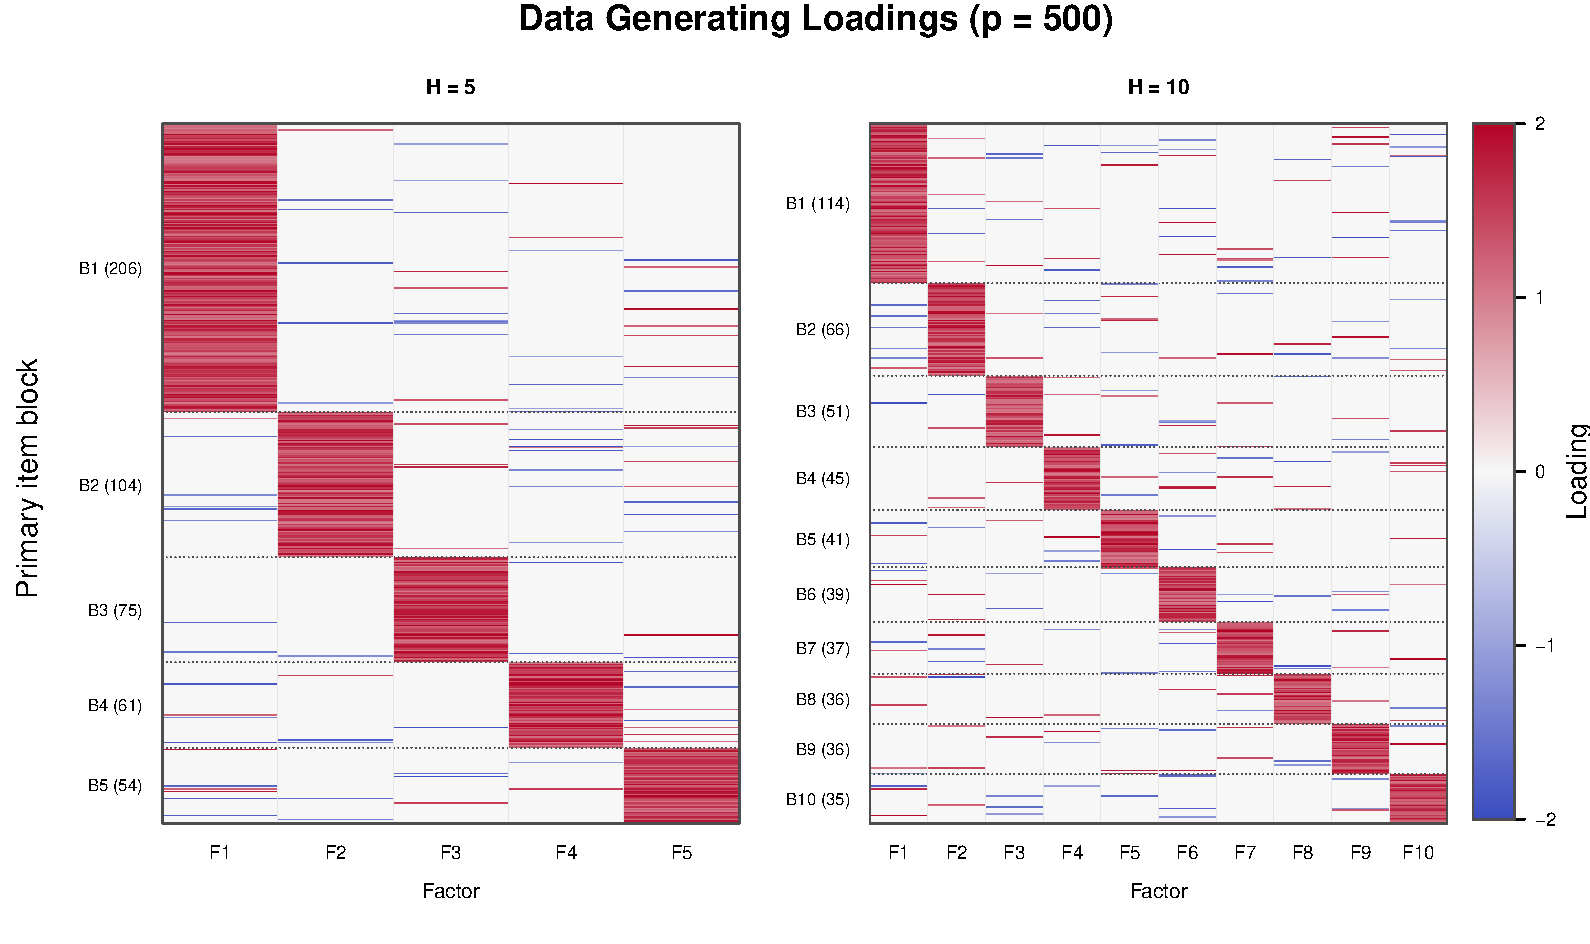
\includegraphics[width=\linewidth]{results/selected_plots/sample_size/paper_simulation_section/fig_data_generating_loadings.pdf}
  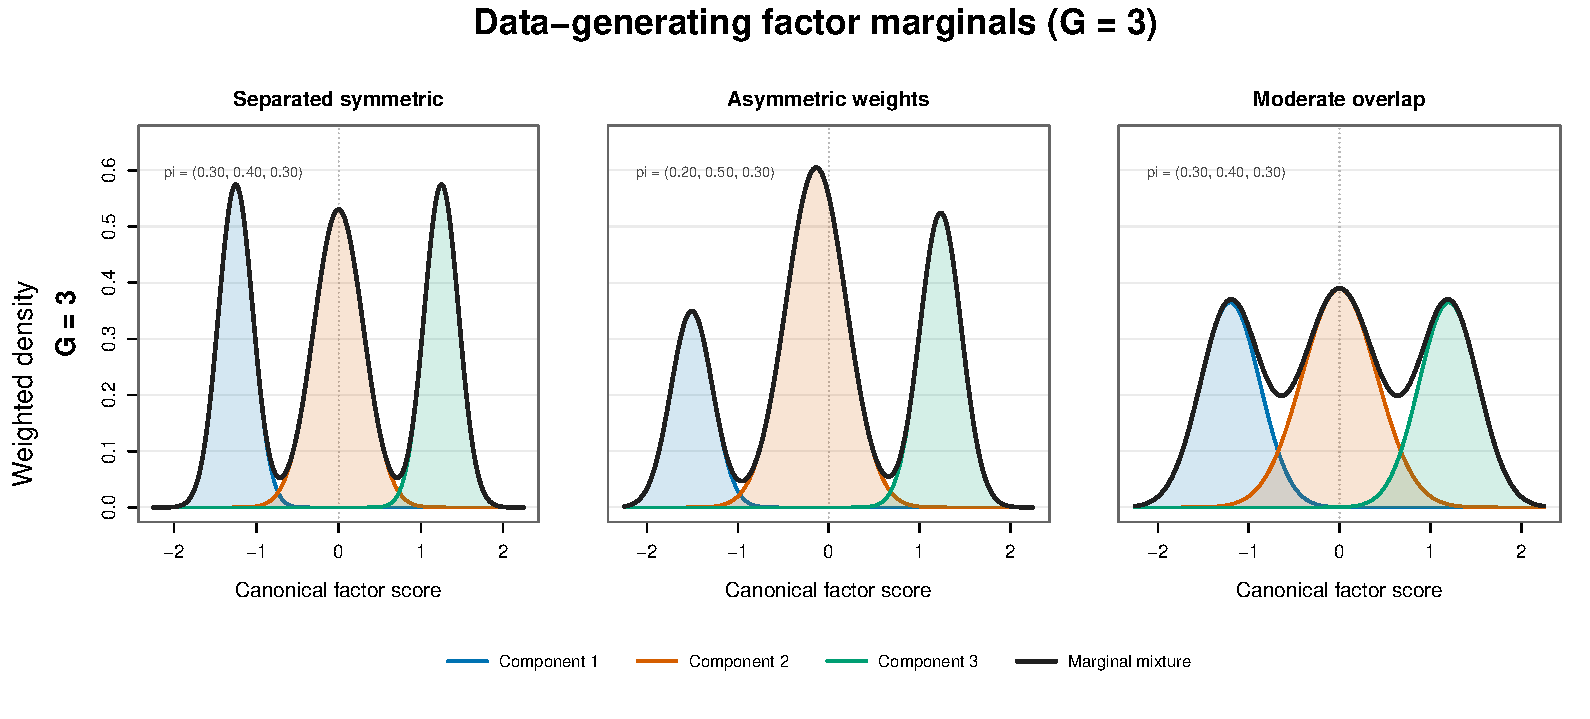
\includegraphics[width=\linewidth]{results/selected_plots/sample_size/paper_simulation_section/fig_data_generating_mixtures.pdf}
  \caption{Data-generating loading structures and factor-mixture distributions.
  Top: sparse, unbalanced loading matrices for $p=500$ and
  $H\in\{5,10\}$. Bottom: representative three-component marginals under the
  separated symmetric, asymmetric-weight, and moderate-overlap
  configurations.}
  \label{fig:loadings_clusters}
\end{figure}

For every combination of $(n,p,H,G_h)$ and mixture configuration, we held the
population loading, intercept, and mixture parameters fixed and independently
generated 25 datasets by redrawing the factors, latent Gaussian responses,
and observed binary responses. Spectral-MAP was run throughout the complete
$p$ grid. Because of its substantially higher cost, Gibbs was run for
$p\in\{500,1000\}$.

Spectral-MAP first estimated the rank-$H$ probit signal by deterministic
EM-SVD. Pretraining stopped when the change in the estimated left singular
subspace fell below $2\times10^{-3}$, the relative loading change fell below
$10^{-4}$, the log-likelihood change fell below $10^{-5}$, or the iteration
limit was reached. The estimated factor subspace was then oriented using a
FastICA initialization followed by Riemannian optimization of the profiled
mixture criterion. Finally, the factor scores, loadings, intercepts, and
marginal mixture parameters were updated by monotone blockwise MAP
refinement. The same Laplace loading penalty was used in pretraining,
rotation, and refinement: $\lambda=3$ when $n=100$ and $\lambda=5$ when
$n\in\{200,400\}$.

The Gibbs comparator used probit augmentation and the Gaussian scale-mixture
representation of the same Laplace loading prior. We ran 2,000 iterations and
discarded the first 1,000 iterations as burn-in. Each retained draw was first
transformed to the canonical factor parameterization and then aligned to a
running loading reference by a globally optimal signed permutation. The same
transformation was applied to factor scores, loadings, component allocations,
and mixture parameters before posterior averaging. This draw-level alignment
prevents factor permutations, sign changes, and component relabeling from
being conflated with posterior uncertainty. The two procedures used the same
mixture priors and loading penalty within each design cell.

Final estimates were canonicalized so that every fitted factor marginal had
mean zero and variance one. We then aligned estimated factors and structural
parameters to the data-generating values and recorded factor-score, loading,
intercept, response-probability, mixture-mean, mixture-variance, and
mixture-weight RMSE. We also recorded end-to-end wall time and, for Gibbs,
effective sample sizes for the aligned parameter traces.

Because subject-level subtyping is a primary use of P-IFA, we evaluated
factor-specific component assignments and the resulting component profile.
For Spectral-MAP, we formed the fitted responsibility
\begin{equation}
\widehat r_{ihg}^{\mathrm{MAP}}
=
\frac{
\widehat\pi_{hg}\,
\phi(\widehat f_{ih};\widehat\mu_{hg},\widehat\sigma_{hg}^{2})
}{
\sum_{\ell=1}^{G_h}
\widehat\pi_{h\ell}\,
\phi(\widehat f_{ih};\widehat\mu_{h\ell},\widehat\sigma_{h\ell}^{2})
},
\qquad
\widehat C_{ih}^{\mathrm{MAP}}
=\arg\max_{1\leq g\leq G_h}\widehat r_{ihg}^{\mathrm{MAP}}.
\label{eq:map_subtype_assignment}
\end{equation}

For Gibbs, we considered two posterior summaries. The allocation-mode
estimator used the most frequently sampled aligned allocation,
\begin{equation}
\widehat C_{ih}^{\mathrm{mode}}
=
\arg\max_{1\leq g\leq G_h}
\frac{1}{S}\sum_{s=1}^{S}
\mathbb{I}\!\left(C_{ih}^{(s)}=g\right),
\label{eq:gibbs_mode_subtype}
\end{equation}
where $S=1000$ is the number of retained draws. The posterior-mean plug-in
estimator first averaged the aligned canonical draws and then classified the
posterior-mean score under the posterior-mean mixture parameters:
\begin{equation}
\overline r_{ihg}
=
\frac{
\overline\pi_{hg}\,
\phi(\overline f_{ih};\overline\mu_{hg},\overline\sigma_{hg}^{2})
}{
\sum_{\ell=1}^{G_h}
\overline\pi_{h\ell}\,
\phi(\overline f_{ih};\overline\mu_{h\ell},\overline\sigma_{h\ell}^{2})
},
\qquad
\widehat C_{ih}^{\mathrm{plug}}
=\arg\max_{1\leq g\leq G_h}\overline r_{ihg}.
\label{eq:gibbs_plugin_subtype}
\end{equation}
The main cross-method comparison uses the allocation-mode Gibbs estimator,
because it directly summarizes the sampled latent allocations; we report the
posterior-mean plug-in estimator as a complementary sensitivity analysis.

Each method yields an individual component profile
$\widehat{\boldsymbol C}_i=(\widehat C_{i1},\ldots,\widehat C_{iH})$.
After aligning component labels within each factor, we measured profile
recovery using Hamming accuracy,
\begin{equation}
\operatorname{Acc}_{\mathrm{Ham}}
=1-
\frac{1}{nH}\sum_{i=1}^{n}\sum_{h=1}^{H}
\mathbb{I}(C_{ih}\neq\widehat C_{ih}).
\label{eq:hammingacc}
\end{equation}
We additionally recorded exact-profile accuracy and factor-specific adjusted
Rand indices.

Figure~\ref{fig:factor_recovery_separated} presents factor recovery under the
separated symmetric configuration. Factor RMSE decreased with $n$ and $p$ for
Spectral-MAP, including the larger-$p$ settings for which Gibbs was not run.
Across the matched $p\in\{500,1000\}$ cells, mean factor RMSE was 0.118 for
Spectral-MAP and 0.120 for Gibbs. Gibbs had a modest advantage in some
small-sample cells, whereas Spectral-MAP was comparable or more accurate in
others. Even at $n=100$, the mean absolute correlation between the estimated
and true Spectral-MAP factors exceeded 0.98 in every $(p,H,G_h)$ cell. Loading
RMSE was also nearly identical after canonicalization, while Gibbs produced
slightly smaller response-probability and intercept RMSE on average.

\begin{figure*}[t]
  \centering
  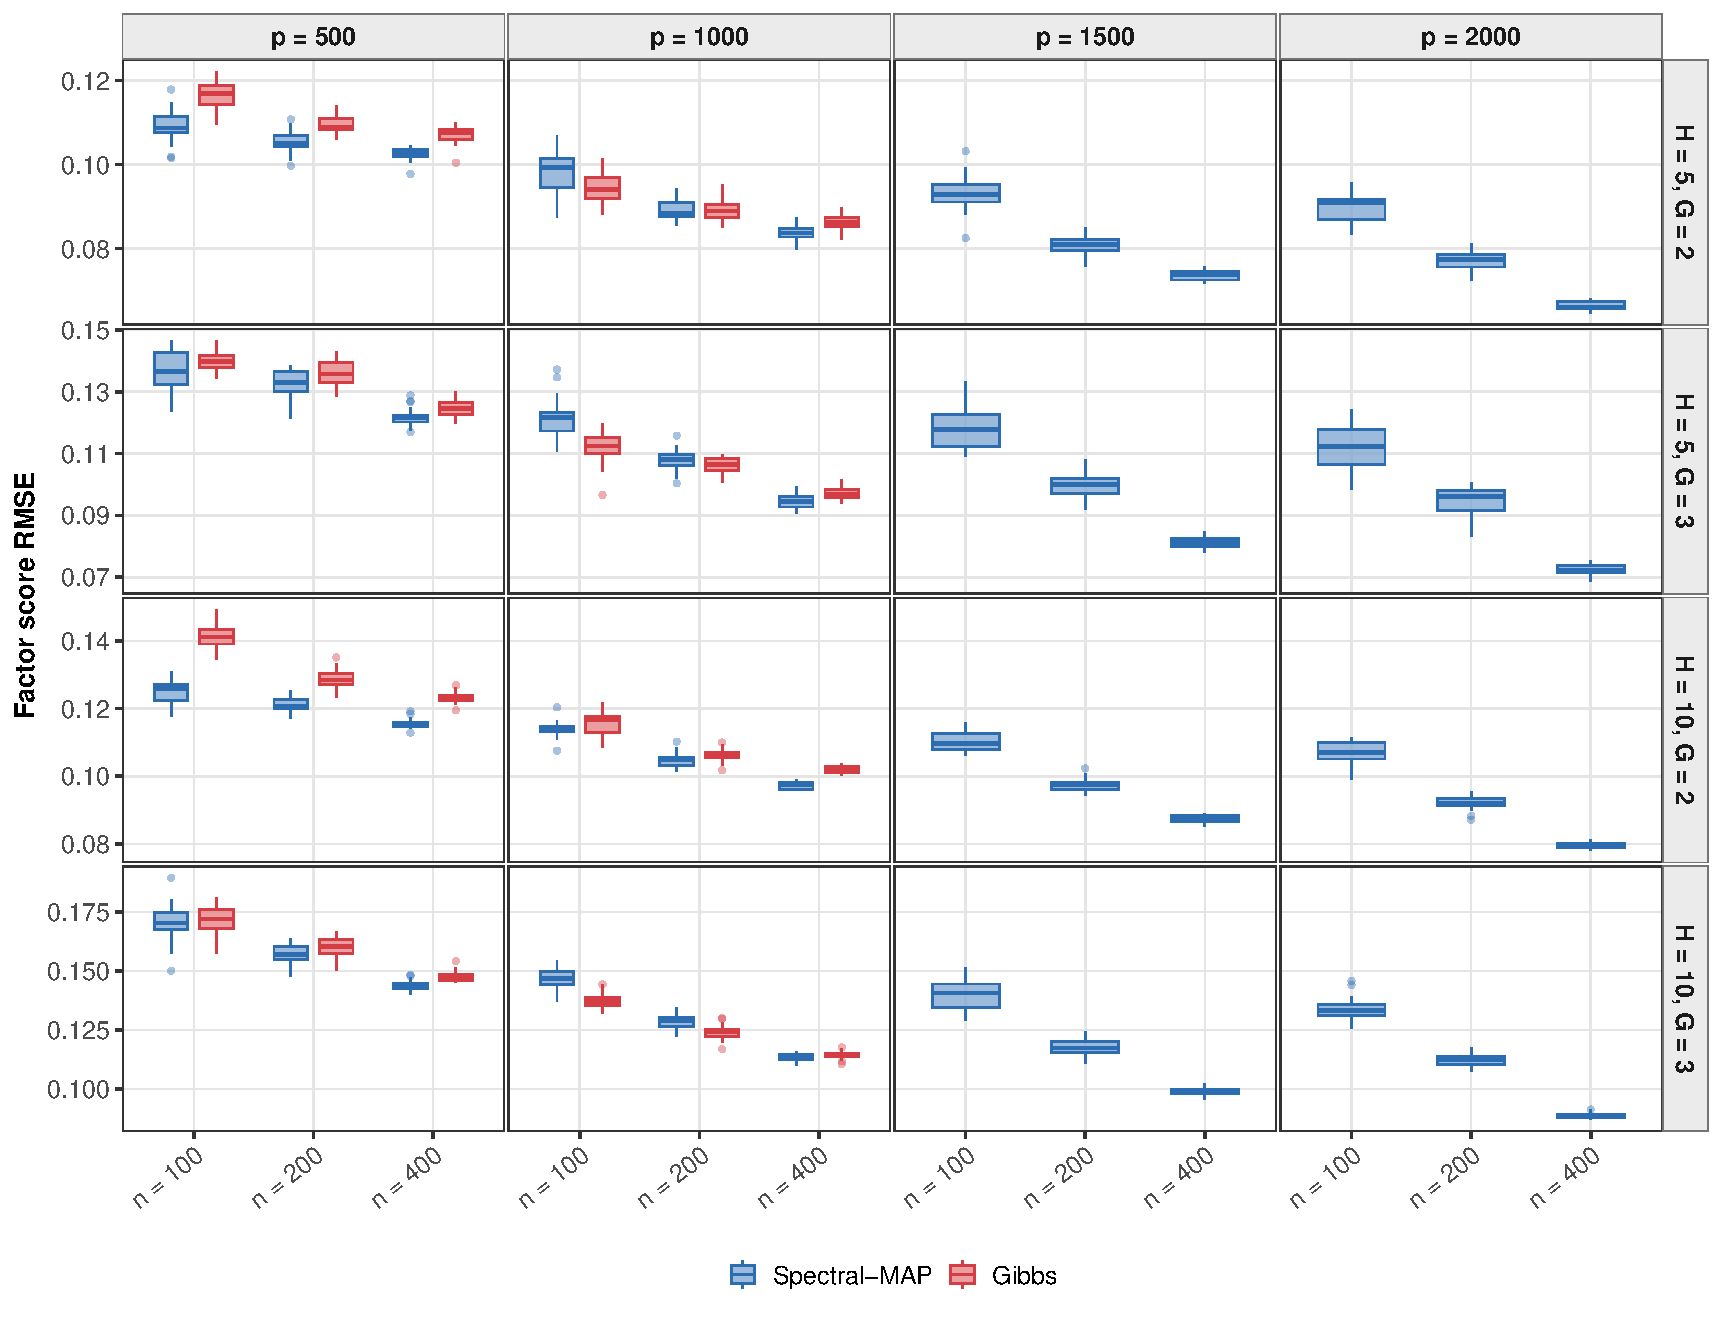
\includegraphics[width=\textwidth]{results/selected_plots/sample_size/paper_simulation_section/fig_factor_recovery_separated.pdf}
  \caption{Factor-score recovery under the separated symmetric mixture
  configuration. Boxplots summarize 25 replications. Gibbs was run for
  $p\in\{500,1000\}$; the $p\in\{1500,2000\}$ columns report Spectral-MAP.}
  \label{fig:factor_recovery_separated}
\end{figure*}

The methods differed more clearly in recovery of the marginal mixture
parameters and component profiles. Figure~\ref{fig:mixture_subtype_separated}
shows that Spectral-MAP generally had lower mixture-mean, mixture-variance,
and mixture-weight RMSE and higher allocation accuracy. Pooled across matched
cells in the separated arm, Spectral-MAP achieved mean RMSEs of 0.076, 0.012,
and 0.037 for the mixture means, variances, and weights, compared with 0.128,
0.136, and 0.044 for Gibbs. Hamming accuracy was 0.987 for Spectral-MAP and
0.938 for the Gibbs allocation-mode estimator.

\begin{figure*}[t]
  \centering
  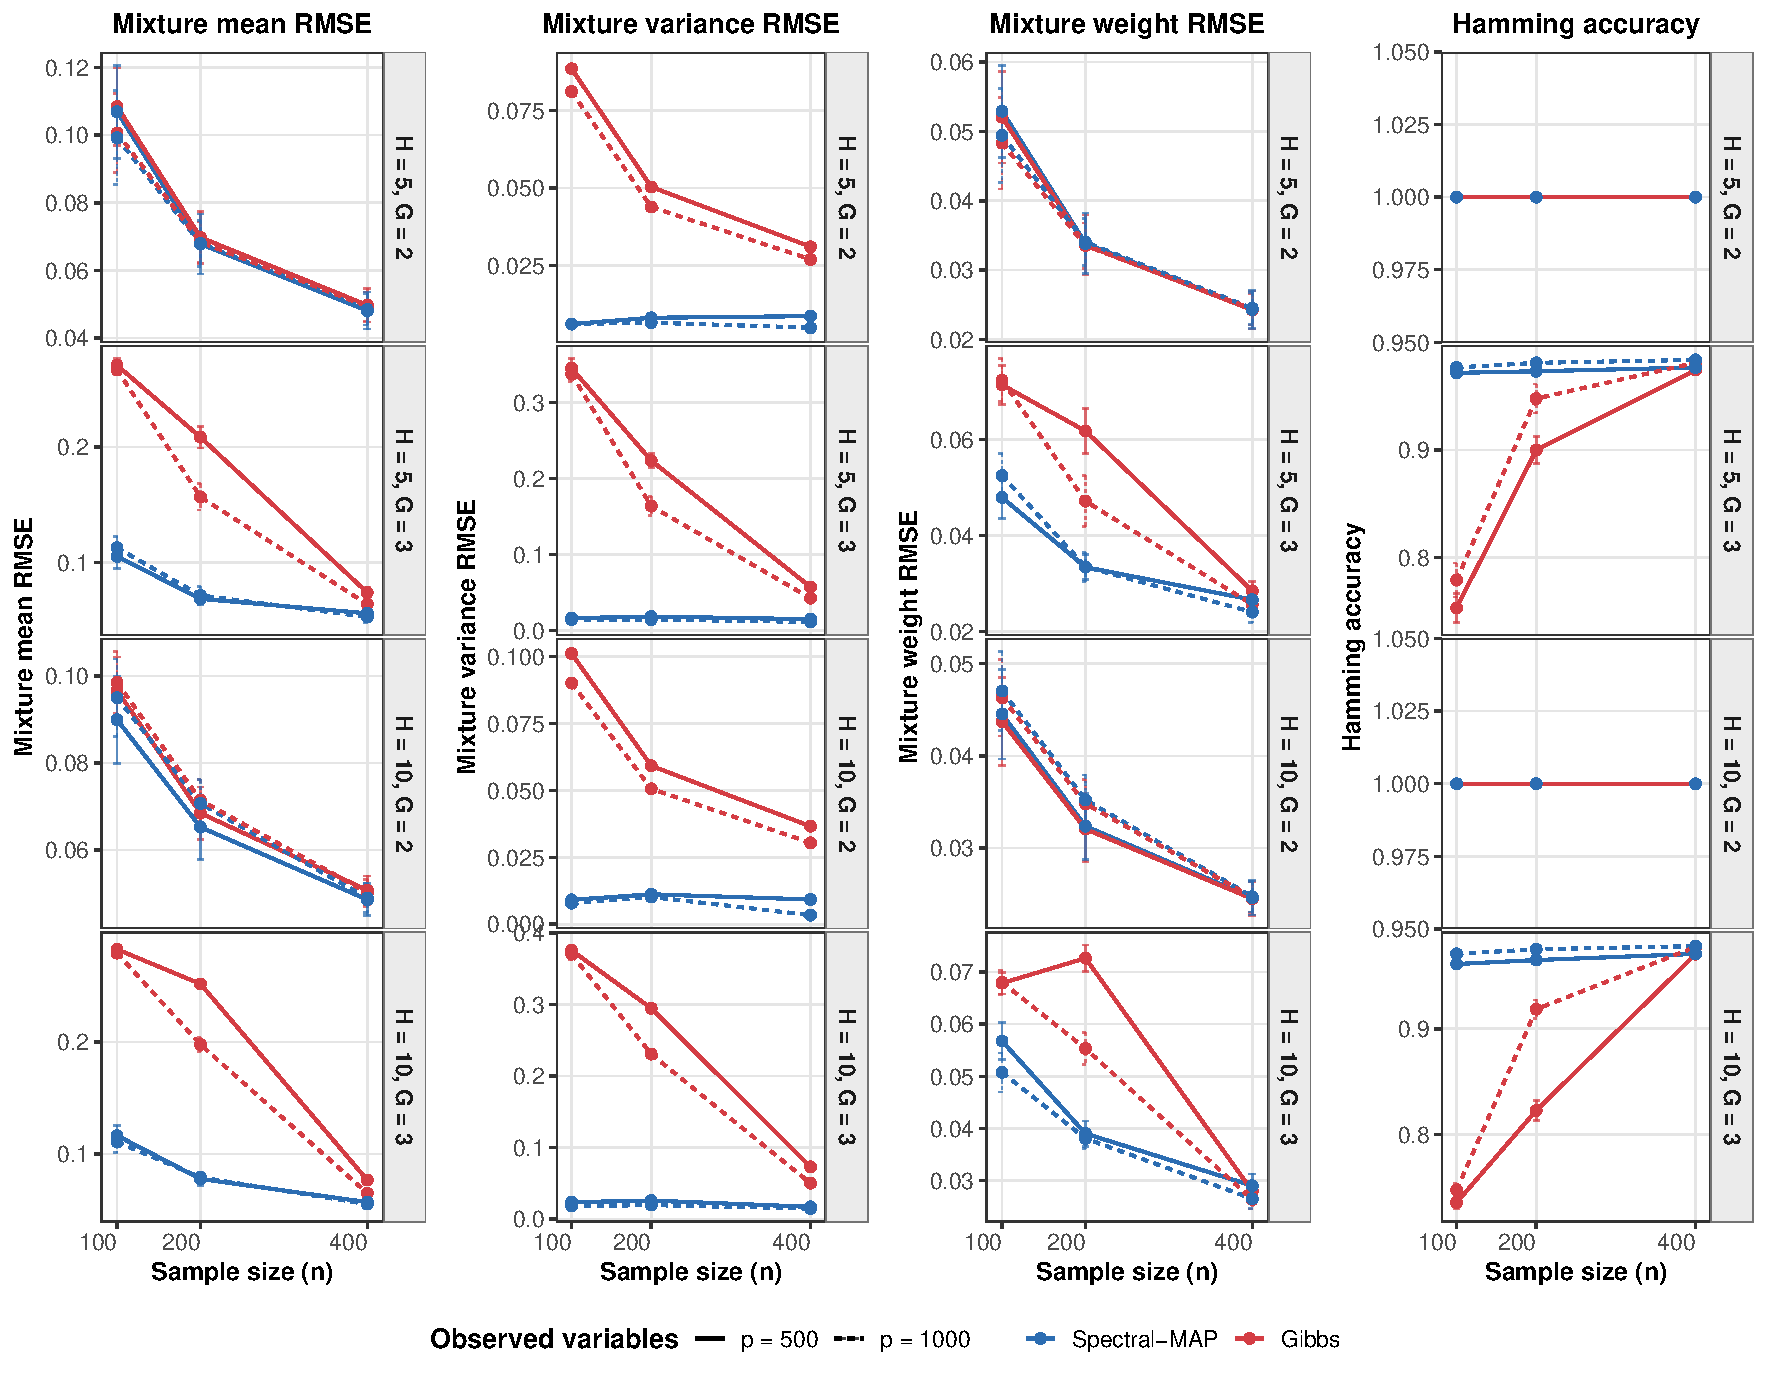
\includegraphics[width=\textwidth]{results/selected_plots/sample_size/paper_simulation_section/fig_mixture_subtype_recovery_separated.pdf}
  \caption{Mixture-parameter and component-profile recovery under the
  separated symmetric configuration. Points are means and bars show
  $\pm2$ Monte Carlo standard errors over 25 replications. Line type
  distinguishes $p=500$ and $p=1000$. The Gibbs Hamming accuracy uses the
  posterior mode of the aligned sampled allocations.}
  \label{fig:mixture_subtype_separated}
\end{figure*}

Table~\ref{tab:subtype_estimators} compares Spectral-MAP with both Gibbs
subtype summaries. The posterior-mean plug-in summary improved Gibbs subtype
recovery relative to the allocation mode: its pooled Hamming accuracy was
0.971 in the separated configuration, 0.968 under asymmetric weights, and
0.923 under moderate overlap, compared with 0.938, 0.943, and 0.877 for the
allocation mode. Spectral-MAP was more accurate than both Gibbs summaries,
with corresponding Hamming accuracies of 0.987, 0.986, and 0.953. Thus, the
subtype advantage is not an artifact of using only one Gibbs summary. The
full parameter and clustering results for all three mixture configurations
are reported in Supplementary Table~\ref{tab:recovery_by_mixture_setting} and
the associated faceted boxplots.

\begin{table}[t]
\centering
\caption{Subtype recovery for Spectral-MAP and two Gibbs posterior summaries. Entries are means with Monte Carlo standard deviations in parentheses, pooled over the matched $p\in\{500,1000\}$ design cells, with 25 replications per cell. The Gibbs allocation-mode estimator uses the modal aligned sampled component label for each subject and factor; the Gibbs posterior-mean plug-in estimator classifies the aligned posterior-mean score using the aligned posterior-mean mixture parameters. Higher values are better.}
\label{tab:subtype_estimators}
\begin{tabular}{llcc}
\toprule
Configuration & Subtype estimator & Hamming & Exact profile \\
\midrule
Separated symmetric & Spectral-MAP plug-in & 0.987 (0.014) & 0.908 (0.111) \\
 & Gibbs allocation mode & 0.938 (0.094) & 0.744 (0.343) \\
 & Gibbs posterior-mean plug-in & 0.971 (0.037) & 0.828 (0.218) \\
\addlinespace
Asymmetric weights & Spectral-MAP plug-in & 0.986 (0.015) & 0.902 (0.118) \\
 & Gibbs allocation mode & 0.943 (0.089) & 0.760 (0.321) \\
 & Gibbs posterior-mean plug-in & 0.968 (0.042) & 0.813 (0.233) \\
\addlinespace
Moderate overlap & Spectral-MAP plug-in & 0.953 (0.048) & 0.742 (0.273) \\
 & Gibbs allocation mode & 0.877 (0.133) & 0.588 (0.425) \\
 & Gibbs posterior-mean plug-in & 0.923 (0.080) & 0.657 (0.357) \\
\bottomrule
\end{tabular}
\end{table}


Spectral-MAP was substantially faster than Gibbs (Table~\ref{tab:runtime_comparison}).
After pooling over $n\in\{100,200,400\}$ and $p\in\{500,1000\}$,
Spectral-MAP was 8.0--11.6 times faster across the four $(H,G_h)$
configurations. Across the 24 individual $(n,p,H,G_h)$ cells, speed-ups ranged
from approximately 5.8 to 15.7. Gibbs effective sample sizes were computed
from the aligned traces, so these timing comparisons include the complete
2,000-draw procedure and its posterior post-processing.

\begin{table}[t]
\centering
\caption{End-to-end computation time under the separated symmetric mixture configuration. Times are means in seconds, pooled over $n\in\{100,200,400\}$ and $p\in\{500,1000\}$, with 25 replications per design cell. Speed-up is the ratio of Gibbs time to Spectral-MAP time. ESS is the mean across replications of the median effective sample size over P-IFA parameters among the 1,000 retained Gibbs draws.}
\label{tab:runtime_comparison}
\begin{tabular}{ccrrrr}
\toprule
$H$ & $G_h$ & Spectral-MAP & Gibbs & Speed-up & Gibbs ESS \\
\midrule
5 & 2 & 20.1 & 161.2 & \textbf{8.0$\times$} & 163 \\
5 & 3 & 15.9 & 161.6 & \textbf{10.2$\times$} & 180 \\
10 & 2 & 26.8 & 218.0 & \textbf{8.1$\times$} & 159 \\
10 & 3 & 18.9 & 218.2 & \textbf{11.6$\times$} & 163 \\
\bottomrule
\end{tabular}
\end{table}


\subsection{Rotation Ablation Study}
\label{sec:rotation_ablation}

We next isolated the contribution of the profiled mixture rotation criterion
in \eqref{eq:penalized_empirical_optim}. To distinguish rotation error from
error in estimating the binary-data signal, this comparison used the oracle
latent Gaussian matrix $\boldsymbol Z$. For each dataset, we extracted the
leading $H$ left singular vectors of $\boldsymbol Z$ and compared three
orientations: FastICA alone; FastICA followed by Riemannian optimization of
the profiled mixture criterion (FastICA + Mixture); and the same mixture
optimization initialized at the identity matrix (Identity + Mixture). Each
rotated score matrix was subsequently passed through the identical MAP
refinement algorithm.

Table~\ref{tab:rotation_ablation_separated} reports post-refinement factor
RMSE for the separated mixture configuration. FastICA + Mixture achieved the
smallest mean RMSE and markedly lower Monte Carlo variability than FastICA
alone. Identity + Mixture also reduced variability, indicating that the
gain is attributable to the mixture-aware objective rather than only to the
FastICA initialization. The asymmetric and moderate-overlap configurations
yielded the same qualitative conclusion; their results are reported in
Supplementary Table~\ref{tab:rotation_ablation_supplement}. These findings
support using FastICA as a convenient initial orientation and the proposed
profiled criterion to identify the orientation most compatible with the
factor-specific Gaussian-mixture model.

\begin{table}[t]
\centering
\caption{Oracle rotation ablation under the well-separated mixture configuration. Entries are post-refinement mean factor-score RMSE with the Monte Carlo standard deviation in parentheses, pooled over all combinations of $n\in\{100,200,400\}$, $p\in\{500,1000,1500,2000\}$, $H\in\{5,10\}$, and $G_h\in\{2,3\}$, with 25 replications per design cell ($1{,}200$ datasets). Lower values are better.}
\label{tab:rotation_ablation_separated}
\begin{tabular}{lc}
\toprule
Rotation strategy & Post-refinement factor RMSE \\
\midrule
FastICA             & $0.124\;(0.074)$ \\
FastICA + Mixture   & $\mathbf{0.109}\;(\mathbf{0.026})$ \\
Identity + Mixture  & $0.118\;(0.058)$ \\
\bottomrule
\end{tabular}
\end{table}

